\documentclass[a4paper,12pt]{article}

\usepackage{mathtext}
\usepackage[T2A]{fontenc}
\usepackage[utf8]{inputenc}
\usepackage[russian]{babel}
\usepackage{multirow}
\usepackage{slashbox}
\usepackage{makecell}
\usepackage{graphicx}
\usepackage{physics}
\usepackage{amstext}
\usepackage{caption}
\usepackage{subcaption}
\usepackage{cmap}
\usepackage{float}


\title{Лабораторная работа 6}
\author{Калашников Михаил, Б03-205}
\date{}


\begin{document}

\maketitle{Изнанка С++}

\begin{enumerate}

\setcounter{enumi}{0}

\item Создадим простой класс.

\begin{figure}[H]
  \centering
  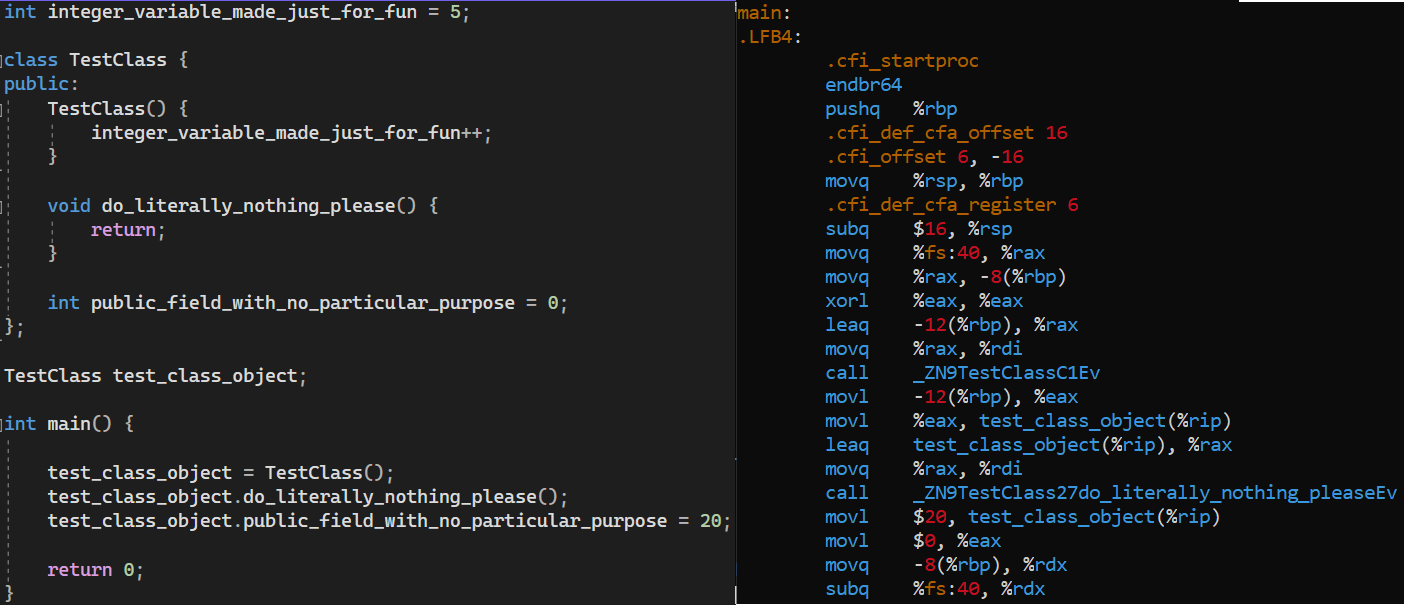
\includegraphics[width=1\linewidth]{images/asm6_1.png}
\end{figure}

Можно увидеть что название метода просто прилепляется к названию класса. Изменение поля выглядит интересно. Обращение к нему происходит через глобальную переменную экземпляра. Реализации класса и метода выглядит как реализация обычных функций.

\begin{figure}[H]
  \centering
  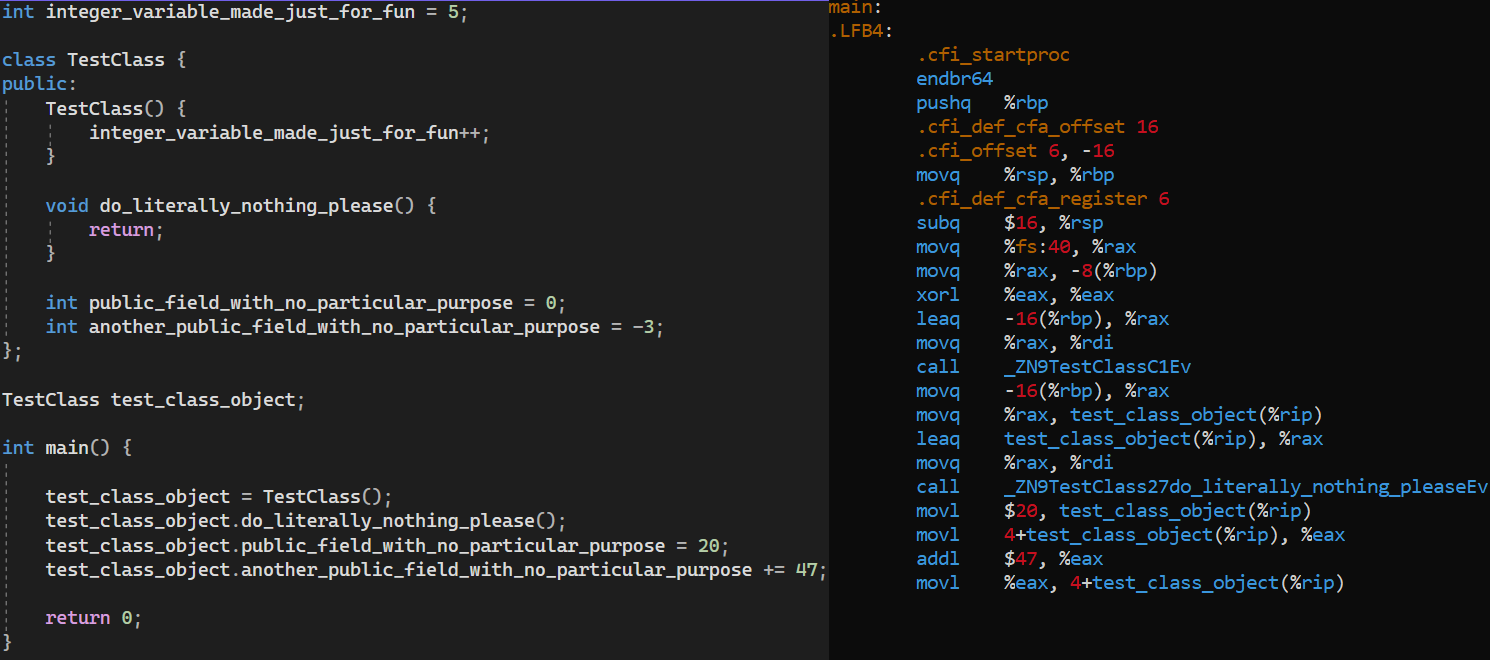
\includegraphics[width=1\linewidth]{images/asm6_2.png}
\end{figure}

Добавив второе поле, можно понять, что поля лежат в памяти друг за другом по адресу экземпляра. В принципе, предсказуемо.

\item Указание на конкретный экземпляр класса происходит через регистр \%rdi. Перед вызовом методов туда складывается адрес нужного объекта и манипуляции в методе происходят уже с ним.

\begin{figure}[H]
  \centering
  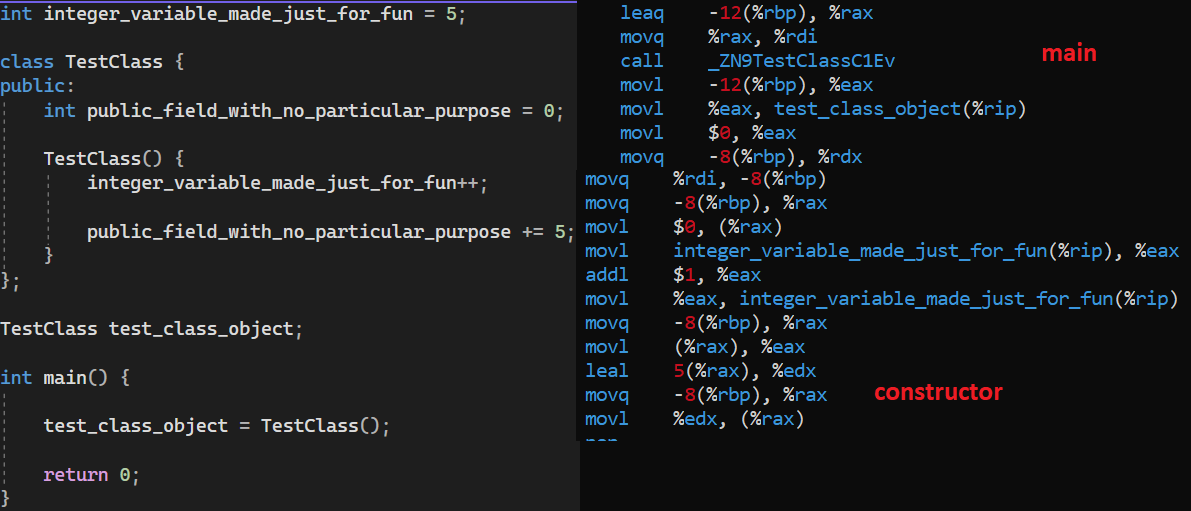
\includegraphics[width=1\linewidth]{images/asm6_3.png}
\end{figure}

\item Добавление слова this не меняет листинг. По сути, this, т.е. указатель на используемый экземпляр, лежит в регистре \%rdi.

\item Что-то вызов дестракторов я не нашел.

\item Приватные и пабликовые методы полностью идентичные. Наличие права обращения к конкретному методу проверяется компилятором, а не в рантайме.

\begin{figure}[H]
  \centering
  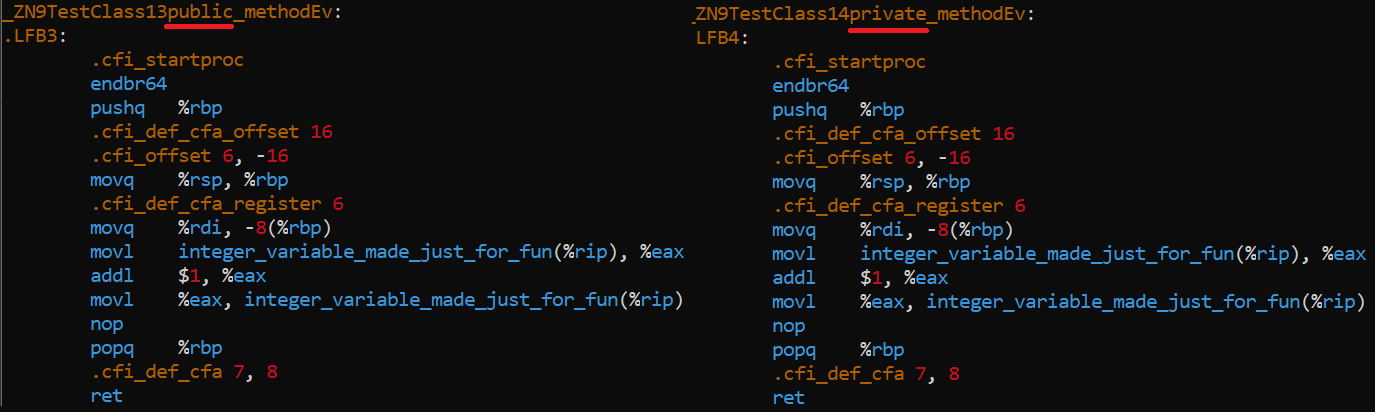
\includegraphics[width=1\linewidth]{images/asm6_4.png}
\end{figure}

\item При наследовании конструкторы вызываются последовательно в обратном порядке, все как рассказывала Катерина Алексеевна в прошлом семестре.

\begin{figure}[H]
  \centering
  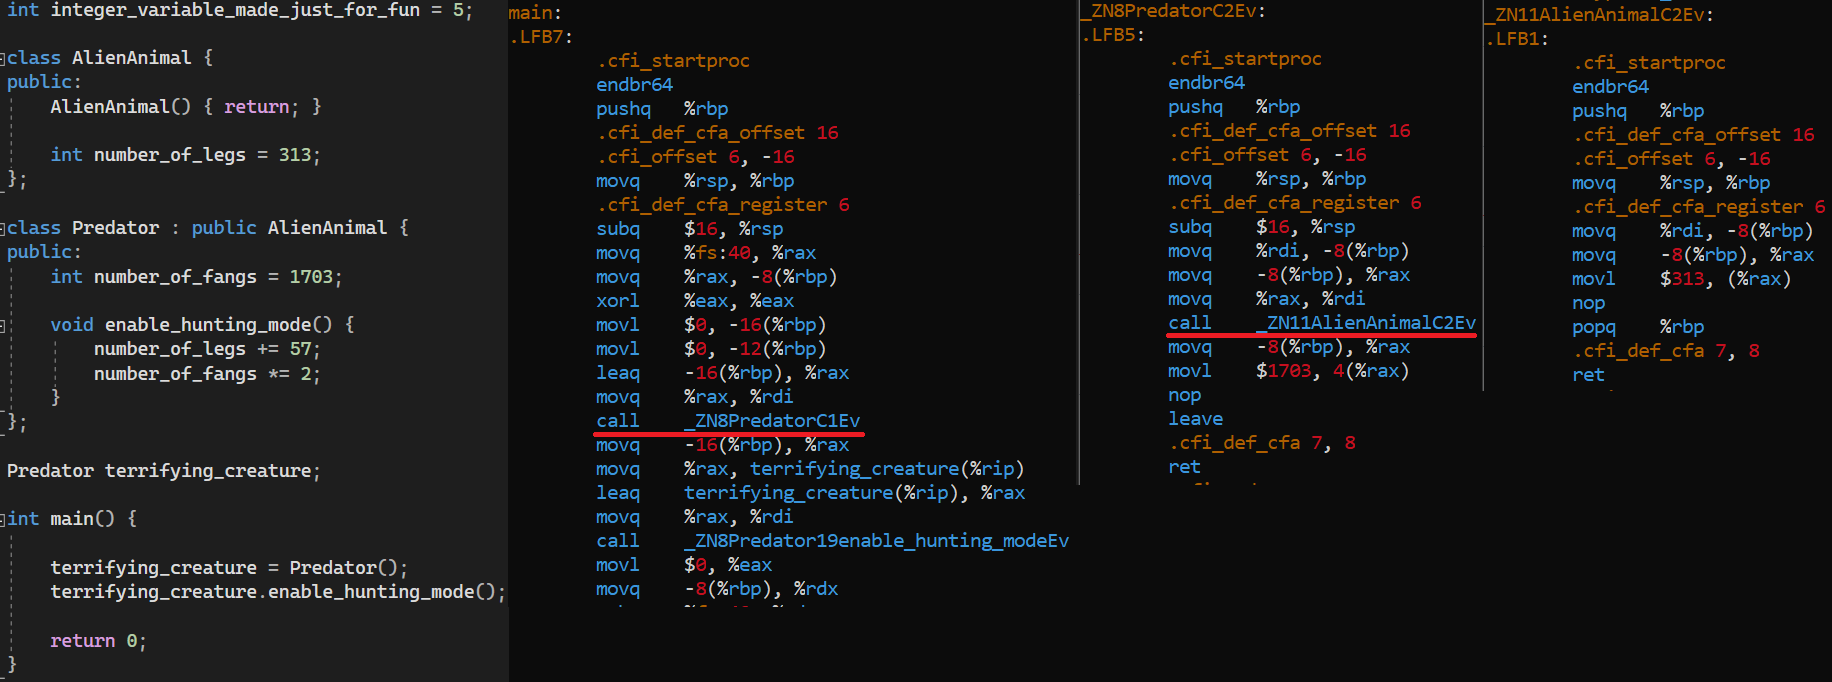
\includegraphics[width=1\linewidth]{images/asm6_5.png}
\end{figure}

\item При полиморфизме компилятор вставляет в листинг вызов метода нужного класса.

\item Работа со статиковыми полями происходит как с глобальными переменными. При вызове статикового метода указатель на экземпляр не запоминается в \%rdi, поэтому метод никак не сможет получить доступ к экземпляру.

\begin{figure}[H]
  \centering
  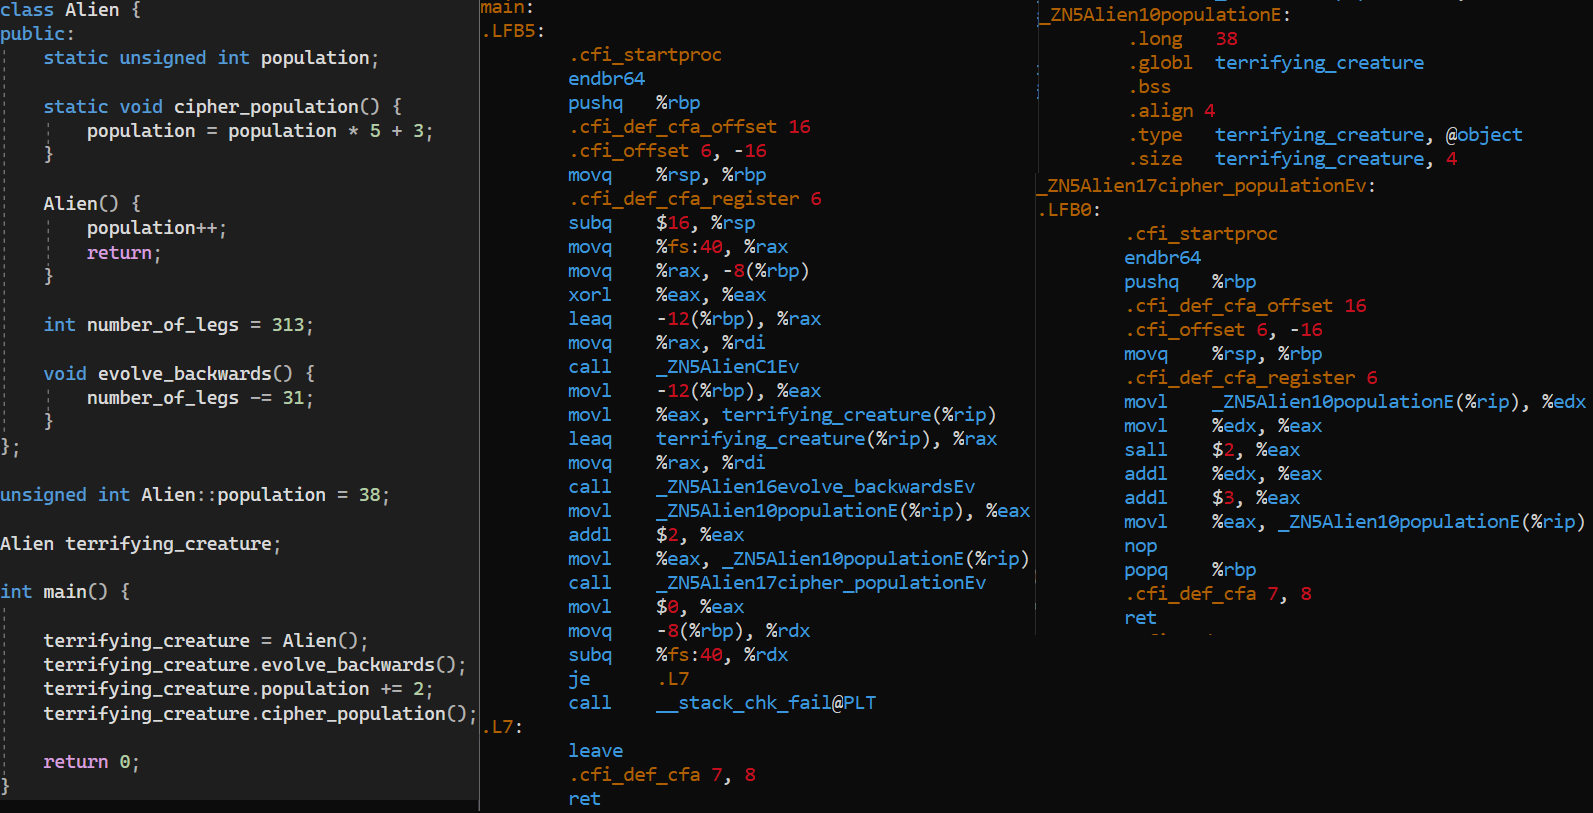
\includegraphics[width=1\linewidth]{images/asm6_6.png}
\end{figure}

\item Перегрузка операторов реализуется очень просто. Создается функция, в название которой входят название класса и перегружаемого оператора (оператор умножения -- ml, сложения -- pl). Потом эта функция вызывается вместо перегруженного оператора.

\item Шаблоны работают максимально предсказуемо. Во время компиляции создаются листинги для каждой требуемой реализации.

\begin{figure}[H]
  \centering
  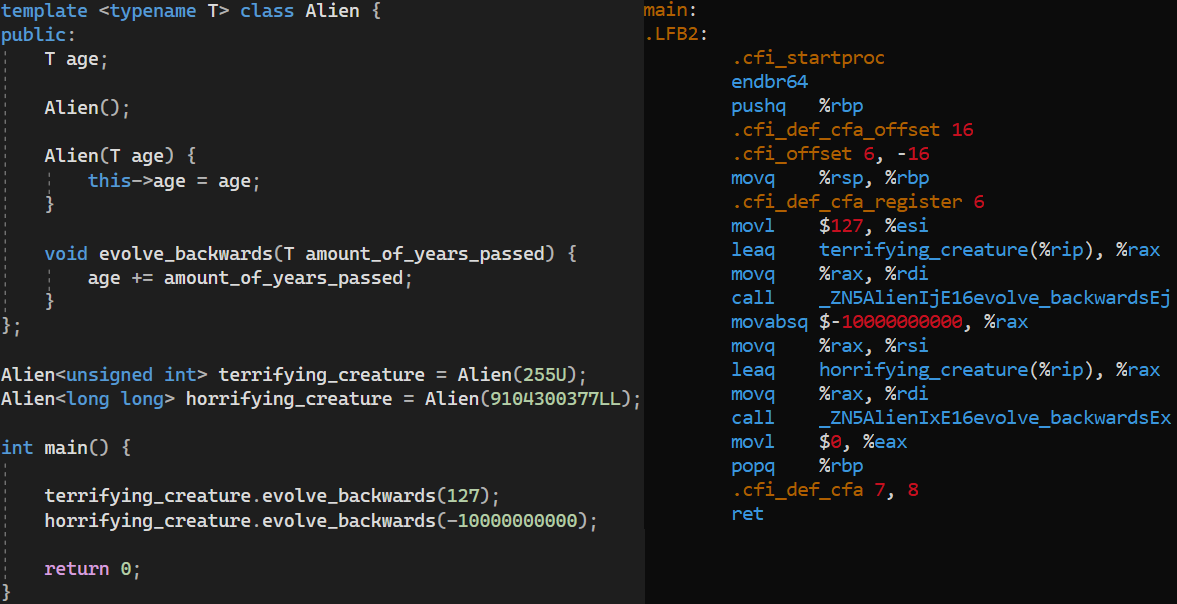
\includegraphics[width=1\linewidth]{images/asm6_7.png}
\end{figure}

\item Enum в принципе работает предсказуемо

\begin{figure}[H]
  \centering
  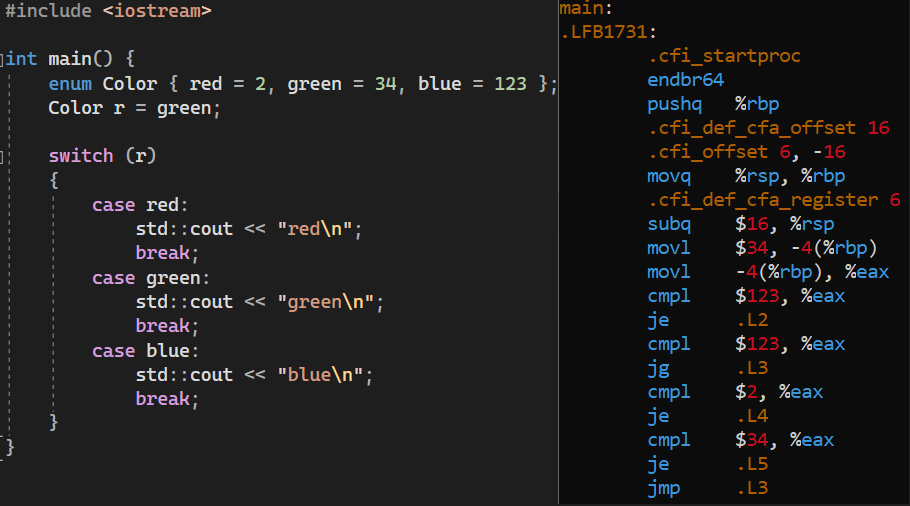
\includegraphics[width=1\linewidth]{images/asm6_8.png}
\end{figure}

\end{enumerate}

\end{document}